
%使用XeLaTeX编译
%版权所有,翻版必究
%本文件由程序自动生成,任何修改将被覆盖
%2019 年 01 月 23 日




\FloatBarrier
\section{
导引
}\label{c000015s000001}


%begin图片
\begin{figure}[htb] %浮动体 here and top ...
%there must use marginnote ...
\marginnote{\setlength\fboxsep{2pt}\fbox{\footnotesize{\kaishu\figurename\,}\footnotesize{\ref{p000012}}}}\centering %中心对齐
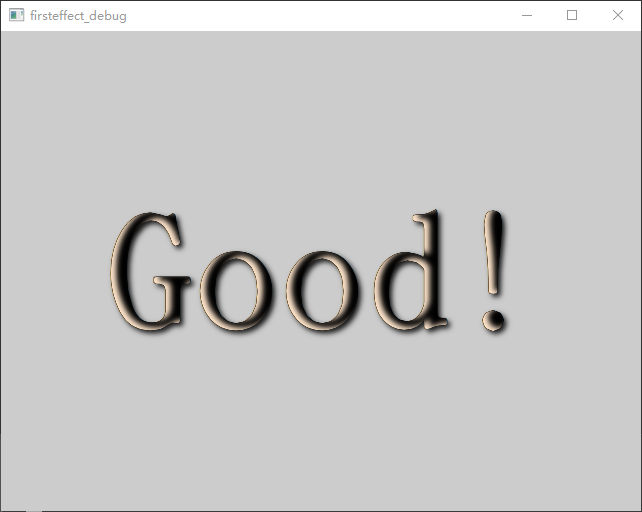
\includegraphics[width=0.95\textwidth]{../chapter06/firsteffect/the_app.png} %图片路径
\caption{文字阴影} %标题
\label{p000012} %索引
\end{figure}
%end图片


aaaaaaaaaaaaaaaaaaaaaaaa
%表
\begin{longtable}{cc}

%表头....
\toprule{}A & B%there must use marginnote ...
\marginnote{\setlength\fboxsep{2pt}\fbox{\footnotesize{\kaishu\tablename\,}\footnotesize{\ref{tb000000}}}}
\\ \midrule 
\endfirsthead

%表尾...
\bottomrule
\caption{ThresholdMask}\label{tb000000} 
\endlastfoot

%重复表头
\toprule{}A & B
\\ \midrule
\endhead
%重复表尾
\midrule
\endfoot 
Blend & aabbc \\
BrightnessContrast & aabbc \\
ColorOverlay & aabbc \\
Colorize & aabbc \\
Desaturate & aabbc \\
GammaAdjust & aabbc \\
HueSaturation & aabbc \\
LevelAdjust & aabbc \\
ConicalGradient & aabbc \\
LinearGradient & aabbc \\
RadialGradient & aabbc \\
Displace & aabbc \\
DropShadow & aabbc \\
InnerShadow & aabbc \\
FastBlur & aabbc \\
GaussianBlur & aabbc \\
MaskedBlur & aabbc \\
RecursiveBlur & aabbc \\
DirectionalBlur & aabbc \\
RadialBlur & aabbc \\
ZoomBlur & aabbc \\
Glow & aabbc \\
RectangularGlow & aabbc \\
OpacityMask & aabbc \\
ThresholdMask  & aabbc \\
\end{longtable}
%表

bbbbbbbbbbbbbbbbbbbbbbbb






%使用XeLaTeX编译
%版权所有,翻版必究
%本文件由程序自动生成,任何修改将被覆盖
%2019 年 01 月 23 日



